% !TEX TS-program = xelatex
% !BIB program = bibtex
% !TEX encoding = UTF-8 Unicode

\documentclass[
  twoside,
  openright,
  degree    = master,               % degree = master | doctor
  language  = english,              % language = chinese | english
  fontset   = template,             % fontset = default | template | system | overleaf
  watermark = true,                 % watermark = true | false
  doi       = false,                 % doi = true | false
]{ntuthesis}

% !TeX root = ./main.tex

% --------------------------------------------------
% 資訊設定(Information Configs)
% --------------------------------------------------

\ntusetup{
  university*   = {National Taiwan University},
  university    = {國立臺灣大學},
  college       = {管理學院},
  college*      = {College of Management},
  institute     = {資訊管理學系},
  institute*    = {Institute of Information Management},
  title         = {基於總體成本與駕駛與乘客間公平性之最佳化共乘演算法},
  title*        = {An Optimization Based Carpool Algorithm in Consideration of the Total Cost and Fairness among the Driver and All Passengers},
  author        = {黃文鴻},
  author*       = {Wen-Hong Huang},
  ID            = {R08725002},
  advisor       = {林永松},
  advisor*      = {Frank Yeong-Sung Lin},
  % date          = {2020-05-01},         % 若註解掉,則預設為當天
  % oral-date     = {2020-05-01},         % 若註解掉,則預設為當天
  % DOI           = {10.5566/NTU2020XXXXX},
  keywords      = {共乘、共享經濟、車輛路徑問題、公平性、斯坦納樹問題、拉格朗日鬆弛法},
  keywords*     = {Carpooling, Sharing economy, Vehicle routing problem, Fairness, Steiner Tree Problem, Lagrangian relaxation},
}

% --------------------------------------------------
% 加載套件(Include Packages)
% --------------------------------------------------

% \usepackage[sort&compress]{natbib}      % 參考文獻
\usepackage{amsmath, amsthm, amssymb}   % 數學環境
\usepackage{ulem, CJKulem}              % 下劃線、雙下劃線與波浪紋效果
\usepackage{booktabs}                   % 改善表格設置
\usepackage{multirow}                   % 合併儲存格
\usepackage{diagbox}                    % 插入表格反斜線
\usepackage{array}                      % 調整表格高度
\usepackage{longtable}                  % 支援跨頁長表格
\usepackage{paralist}                   % 列表環境


\usepackage{lipsum}                     % 英文亂字
\usepackage{zhlipsum}                   % 中文亂字

% --------------------------------------------------
% 套件設定(Packages Settings)
% --------------------------------------------------


\begin{document}

% 封面與口試審定
% Cover and Verification Letter
\makecover                          % 論文封面(Cover)
% \makeverification                   % 口試委員審定書(Verification Letter)

% 致謝與論文摘要
% Acknowledgement and Abstract
% % !TeX root = ../main.tex

\begin{acknowledgement}

常到外國朋友家吃飯。當蠟燭燃起,菜肴布好,客主就位,總是主人家的小男孩或小女孩舉起小手,低頭感謝上天的賜予,並歡迎客人的到來。

我剛到美國時,常鬧得尷尬。因為在國內養成的習慣,還沒有坐好,就開動了。

以後凡到朋友家吃飯時,總是先囑咐自己;今天不要忘了,可別太快開動啊!幾年來,我已變得很習慣了。但我一直認為只是一種不同的風俗儀式,在我這方面看來,忘或不忘,也沒有太大的關係。

前年有一次,我又是到一家去吃飯。而這次卻是由主人家的祖母謝飯。她雪白的頭髮,顫抖的聲音,在搖曳的燭光下,使我想起兒時的祖母。那天晚上,我忽然覺得我平靜如水的情感翻起滔天巨浪來。

在小時候,每當冬夜,我們一大家人圍著個大圓桌吃飯。我總是坐在祖母身旁。祖母總是摸著我的頭說:「老天爺賞我們家飽飯吃,記住,飯碗裡一粒米都不許剩,要是蹧蹋糧食,老天爺就不給咱們飯了。」

剛上小學的我,正在念打倒偶像及破除迷信等為內容的課文,我的學校就是從前的關帝廟,我的書桌就是供桌,我曾給周倉畫上眼鏡,給關平戴上鬍子,祖母的話,老天爺也者,我覺得是既多餘,又落伍的。

不過,我卻很尊敬我的祖父母,因為這飯確實是他們掙的,這家確實是他們立的。我感謝面前的祖父母,不必感謝渺茫的老天爺。

這種想法並未因為年紀長大而有任何改變。多少年,就在這種哲學中過去了。

我在這個外國家庭晚飯後,由於這位外國老太太,我想起我的兒時,由於我的兒時,我想起一串很奇怪的現象。

祖父每年在「風裡雨裡的咬牙」,祖母每年在「茶裡飯裡的自苦」,他們明明知道要滴下眉毛上的汗珠,才能撿起田中的麥穗,而為什麼要謝天?我明明是個小孩子,混吃混玩,而我為什麼卻不感謝老天爺?

這種奇怪的心理狀態,一直是我心中的一個謎。

一直到前年,我在普林斯頓,瀏覽愛因斯坦的我所看見的世界得到了新的領悟。

這是一本非科學性的文集,專載些愛因斯坦在紀念會上啦,在歡迎會上啦,在朋友的喪禮中,他所發表的談話。

我在讀這本書時忽然發現愛因斯坦想盡量給聽眾一個印象:即他的貢獻不是源於甲,就是由於乙,而與愛因斯坦本人不太相干似的。

就連那篇亙古以來嶄新獨創的狹義相對論,並無參考可引,卻在最後天外飛來一筆,「感謝同事朋友貝索的時相討論。」

其他的文章,比如奮鬥苦思了十幾年的廣義相對論,數學部份推給了昔年好友的合作:這種謙抑,這種不居功,科學史中是少見的。

我就想,如此大功而竟不居,為什麼?像愛因斯坦之於相對論,像我祖母之於我家。

幾年來自己的奔波,做了一些研究,寫了幾篇學術文章,真正做了一些小貢獻以後,才有了一種新的覺悟:即是無論什麼事,得之於人者太多,出之於己者太少。因為需要感謝的人太多了,就感謝天罷。無論什麼事,不是需要先人的遺愛與遺產,即是需要眾人的支持與合作,還要等候機會的到來。越是真正做過一點事,越是感覺自己的貢獻之渺小。

於是,創業的人,都會自然而然的想到上天,而敗家的人卻無時不想到自己。

\end{acknowledgement}       % 致謝(Acknowledgement)
% !TeX root = ../main.tex

\begin{abstract}

共享經濟是隨著網路以及行動裝置普及下逐漸興起的熱潮,傳統的計程車與共乘服務在共享經濟的風潮下產生出新的商業模式,不同於以往使用者必須到目的地才能知道價錢,或是只能針對特定路線如通勤、通學等才容易有共乘機會;透過線上叫車服務,使用者除了可以事先知道價錢,還可以透過共乘配對服務,自動配對有相近路線的乘客,共同分攤車資,提供使用者更便宜經濟的選擇。

目前的線上共乘配對服務,為共乘平台針對目前行徑中或是配對中的乘客透過運算,找尋最適合的路線與乘客。自動配對的共乘服務中,往往需要多繞路以同時滿足不同乘客間的載運需求,如何讓使用者之間繞路多寡符合公平性,便是重要的挑戰。本研究考慮共享經濟中共乘服務的多乘客路線規劃問題,將乘客可接受的抵達時間、繞多少路的可接受程度,車輛人數限制,以及載客的優先順序納入考量,以最小化最大乘客共乘後節費比例,透過拉格朗日鬆弛法以取得最佳解。

\end{abstract}

\begin{abstract*}

\end{abstract*}              % 摘要(Abstract)

% 生成目錄與符號列表
% Contents of Tables and Denotation
\maketableofcontents                % 目錄(Table of Contents)
\makelistoffigures                  % 圖目錄(List of Figures)
\makelistoftables                   % 表目錄(List of Tables)
% % !TeX root = ../main.tex

\begin{denotation}[3cm]

\item[HPC]{
  高性能計算 (High Performance Computing)
}

\item[cluster]{
  集群
}

\item[Itanium]{
  安騰
}

\item[SMP]{
  對稱多處理
}

\item[API]{
  應用程序編程接口
}

\item[PI]{
  聚酰亞胺
}

\item[MPI]{
  聚酰亞胺模型化合物,N-苯基鄰苯酰亞胺
}

\item[PBI]{
  聚苯並咪唑
}

\item[MPBI]{
  聚苯並咪唑模型化合物,N-苯基苯並咪唑
}

\item[PY]{
  聚吡嚨
}

\item[PMDA-BDA]{
  均苯四酸二酐與聯苯四胺合成的聚吡嚨薄膜
}

\item[$\Delta G$]{
  活化自由能 (Activation Free Energy)
}

\item[$\chi$]{
  傳輸系數 (Transmission Coefficient)
}

\item[$E$]{
  能量
}

\item[$m$]{
  質量
}

\item[$c$]{
  光速
}

\item[$P$]{
  概率
}

\item[$T$]{
  時間
}

\item[$v$]{
  速度
}

\item[勸學]{
  君子曰:學不可以已。青,取之於藍,而青於藍;冰,水為之,而寒於水。木直中繩。輮以為輪,其曲中規。雖有槁暴,不覆挺者,輮使之然也。故木受繩則直,金就礪則利,君子博學而日參省乎己,則知明而行無過矣。吾嘗終日而思矣,不如須臾之所學也;吾嘗跂而望矣,不如登高之博見也。登高而招,臂非加長也,而見者遠;順風而呼,聲非加疾也,而聞者彰。假輿馬者,非利足也,而致千裏;假舟楫者,非能水也,而絕江河,君子生非異也,善假於物也。積土成山,風雨興焉;積水成淵,蛟龍生焉;積善成德,而神明自得,聖心備焉。故不積跬步,無以至千裏;不積小流,無以成江海。騏驥一躍,不能十步;駑馬十駕,功在不舍。鍥而舍之,朽木不折;鍥而不舍,金石可鏤。蚓無爪牙之利,筋骨之強,上食埃土,下飲黃泉,用心一也。蟹六跪而二螯,非蛇鱔之穴無可寄托者,用心躁也。—— 荀況
}

\end{denotation}
            % 符號列表(Denotation)

% 論文內容
% Contents of Thesis
\mainmatter
% !TeX root = ../main.tex

\chapter{Introduction}

\section{Background}

近年來,隨著網際網路的普及以及幾乎人手一支的行動裝置帶動之下,資訊分享無遠弗屆,開始有人將閒置資源放到網路上與人們共享與交換,然而與陌生人共享意味者風險,隨著使用者評比系統的出現,共享平台開始可以透過評比知道使用者好壞,大大降低了網路共享行為的風險\cite{schor_debating_2014},此後這樣的共享平台逐漸推廣到生活的各個層面,蔚為風潮,從食物外送、住宿、乘車都可以見到他的身影,而人們稱呼這樣的新模式為「共享經濟」。

如何定義共享經濟目前並沒有統一的說法,一般來說,共享經濟中的活動主要分為四大類型:商品的再循環、增加耐久財的使用率、服務交換與經營性資產的共享\cite{schor_debating_2014}。這些活動本質上圍繞著「閒置資產」的重新分配\cite{frenken_smarter_2015},不論是透過資源的交換,或從中賺取報酬,只要透過共享經濟平台的媒合,低廉的交易成本使得閒置資產擁有者將資產發揮更大的價值,而需求者能以較低廉的成本運用該資產,如此一來便能增進整體社會資產的使用率,甚至可以「以租代買」,改變以往必須擁有資產才能使用的思維。

共享經濟的閒置資產重新分配精神,為行之有年的計程車與共乘服務注入了活水,相對於傳統的大眾運輸服務,共享經濟下的新型態的運輸服務有以下的特色:
  
1. 有效率的資源使用:傳統的計程車以往需要透過路邊攔車、電話叫車或是計程車隊的無線電派車模式,以台灣為例,根據交通部數據,巡迴攬客、招呼站等候以及定點排班\cite{noauthor_100nianjichengcheyingyunzhuangkuangdiaochabaogao_2012}便佔了超過一半的比例,這樣的叫車模式,需要計程車在路上徘徊,或是在定點等候,容易增加計程車的時間空車率,造成資源浪費;透過叫車平台的派車服務,可以隨時媒合平台上的計程車,使用者也不須在路邊等候,只需要打開手機,便可明確知道計程車抵達時間,旅程時間,減少不確定性同時也可以提升計程車使用率。
2. 動態的服務資源:叫車平台上的司機可彈性決定自己的工作時間,隨時可以透過登入與登出叫車App,決定是否開放載客,因此相對於傳統無線電計程車有固定的派車資源,叫車平台的供給方有非常高度的動態性。
3. 動態共乘:有些叫車App也提供共乘配對服務,如UberPool與Lyft Line,只要開啟App中的共乘選項,便能及時配對有相近路線需求的乘客,不但可以一起分攤車資,還可以減少旅程中空位的浪費,然而對於平台設計者而言,如何在動態的路線需求中,規劃出能滿足各乘客的行車路線,並在媒合各乘客路線的同時,能有合理範圍的繞路。

從以上特性中,我們可以了解到,在新型態的叫車平台上,不論供需雙方都具有高度的動態性與不確定性,在叫車平台上的共乘服務,還需考量隨時從各地出現的路線需求中,找到合適的司機規劃出適合的路線,這對平台方來說,會是一大考驗。

\section{Motivation}

In the early, ride-sharing was necessary to go carpooling by matching at a taxi station, a fixed commuter route or self-organized among people who knew each other \cite{chan_ridesharing_2012}. With the maturity of mobile devices, they are widely used in every corner of life, such as food, clothing, housing, and transportation. Carpooling is a classic example. In the sharing economy era, when one takes out his/her mobile phone, the ride-sharing service can make better use of the "idle assets" such as seats and vehicles. Drivers can now earn more by detour s for ride-sharing. Riders can share the fare with others at a cost-effective price.

However, a trip may consist of many riders with different origins and destinations; charging riders with fairness is a big problem. There are detours and waiting times among the riders, which may be varied. Some people likely detour a lot in a shared ride, and some people hardly detour but have to pay a similar fare. It is very unfair for the riders in the same carpooling. Therefore, making it fair between passengers in the ride-sharing problem is the object of this article.

\section{Objective}

This research aims to maximize the minimal percentage of cost-saving between a rider choose to hail a ride on his/her own and go carpooling. In order to ensure there is no significant deviation from what a rider expects. Constraints are applied with a ride request of origin and destination, car capacity, and detour limitation.

\section{Thesis Organization}

The rest of the paper is organized as follows. We will go through the related work of the carpooling problem in Chapter 2. Chapter 3 will describe the carpooling problem in detail and formulate it into a mathematical model.
% !TeX root = ../main.tex

\chapter{Literature Review}

\section{Related research on carpooling}

\section{Dial-a-ride-problem}

\section{Steiner tree}

In order
% !BIB program = bibtex
% !TeX root = ../main.tex

\chapter{Problem Formulation}

In this chapter, we will introduce the scenario of the carpooling fairness problem. Then formulate the problem into a mathematical model with given parameters and decision variables.

\section{Problem Description}

The object of this research is to minimize the maximum percentage of cost saving when a passenger chooses to carpool, with consideration of the number of drivers, car capacity and routing limit constraints.

Take Figure 3-1 as an example scenario; Passenger 1 and Passenger 2 are requesting a trip. When Passenger 1 chooses to take a ride by himself/herself, called "exclusive" riding shown as Figure 3-2, it would cost \$5. We can describe the scenario as a shortest path problem from $S$ to $D_1$, and $P_1$ is a must-pass node. We use Steiner tree to solve this kind of shortest path problem with must-pass nodes. Passenger 2's "exclusive" riding would also cost \$5 in Figure 3-3. In this case, it would be a shortest path problem from $S$ to $D_2$ with $P_2$ as a must-pass node.

When the passengers choose to take a carpool, which is called "sharing" riding. We can describe the scenario as a shortest problem from $S$ to $D_1$ with $P_1$, $P_2$ and $D_2$ as must-pass nodes or $S$ to $D_2$ with $P_1$, $P_2$ and $D_1$ as must-pass nodes. In Figure 3-4 is one of the best case, which would cost \$8 for all the passengers, in Figure 3-5 would cost the same \$8 and both of the fares they could share are \$5 ( $\overline{P_2D_1}$ and $\overline{P_2D_2}$ respectively); however, in Figure 3-4 would cost $\overset{\overline{P_1P_2}}{1} + \frac{1}{2} \times \overset{\overline{P_2D_1}}{5} = \$3.5$ for Passenger 1 and $\frac{1}{2} \times \overset{\overline{P_2D_1}}{5} + \overset{\overline{D_1D_2}}{1} = \$3.5$ for Passenger 2, in Figure 3-5 would cost $\overset{\overline{P_1P_2}}{1} + \frac{1}{2} \times \overset{\overline{P_2D_2}}{5} + \overset{\overline{D_2D_1}}{1} = \$4.5$ for Passenger 1 and $\frac{1}{2} \times \overset{\overline{P_2D_2}}{5} = \$2.5$ for Passenger 2.

\begin{figure}[htp]
  \centering
  \captionsetup{justification=centering}
  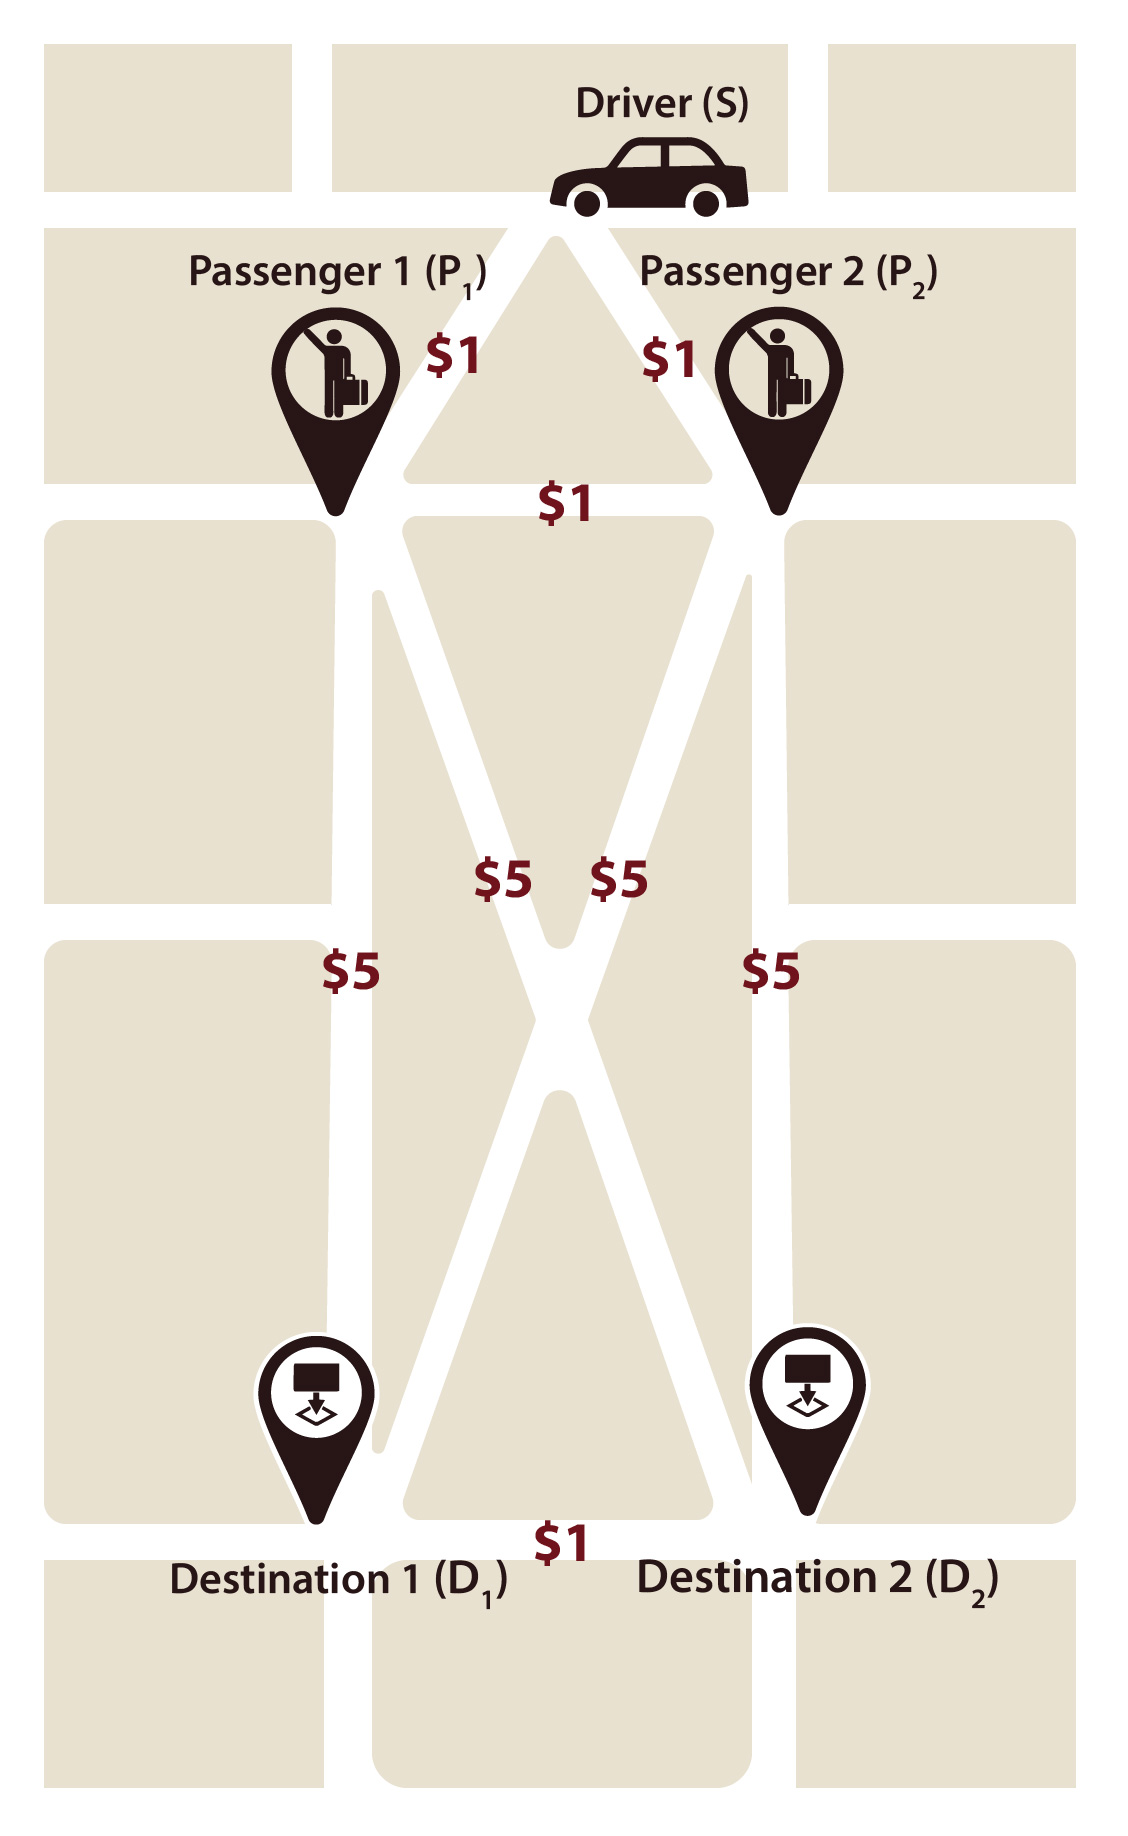
\includegraphics[width=6cm]{figures/mapV2.jpg}
  \caption{Example road network with driving fare and points of passengers and their destinations}
\end{figure}

\begin{figure}[htp]
  \centering
  \captionsetup{justification=centering}
  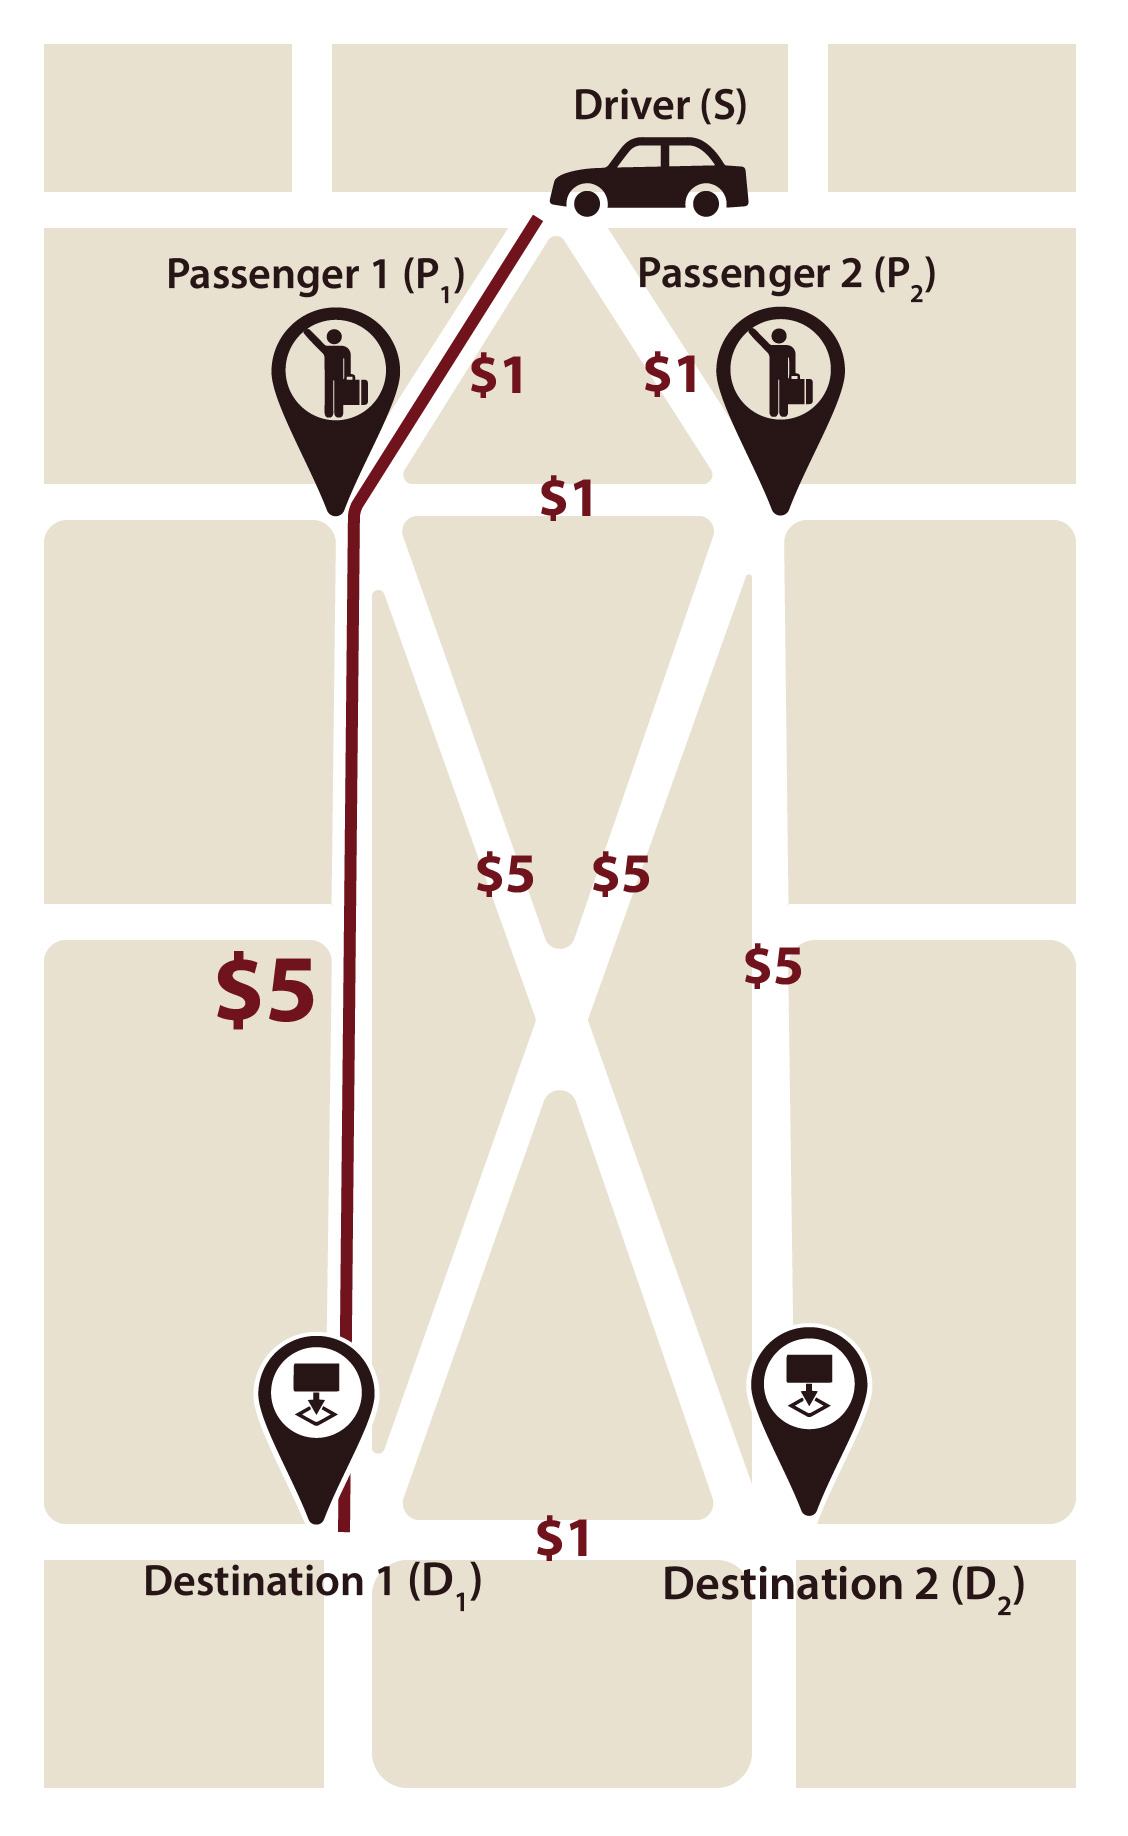
\includegraphics[width=6cm]{figures/mapV2_1.jpg}
  \caption{Best routing path when the driver only serving Passenger 1}
\end{figure}

\begin{figure}[htp]
  \centering
  \captionsetup{justification=centering}
  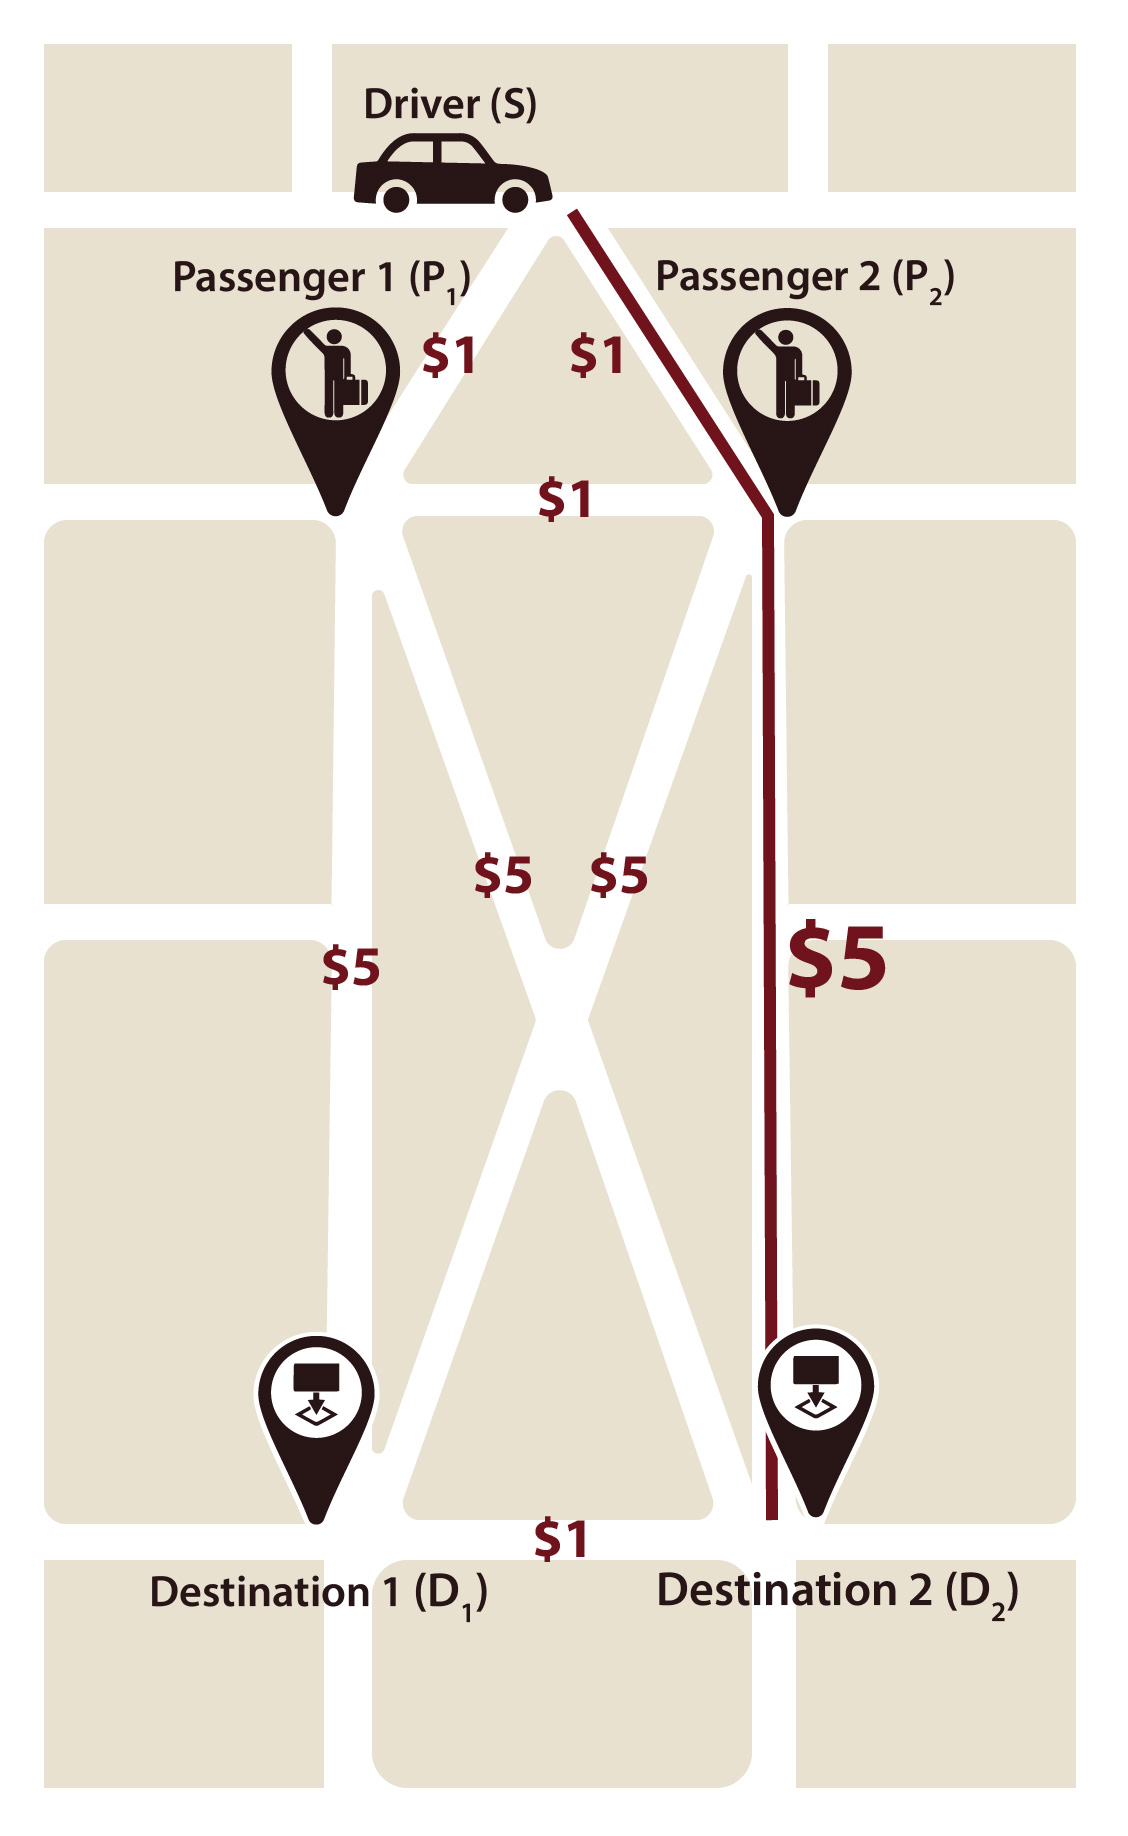
\includegraphics[width=6cm]{figures/mapV2_4.jpg}
  \caption{Best routing path when the driver only serving Passenger 2}
\end{figure}

\begin{figure}[htp]
  \centering
  \captionsetup{justification=centering}
  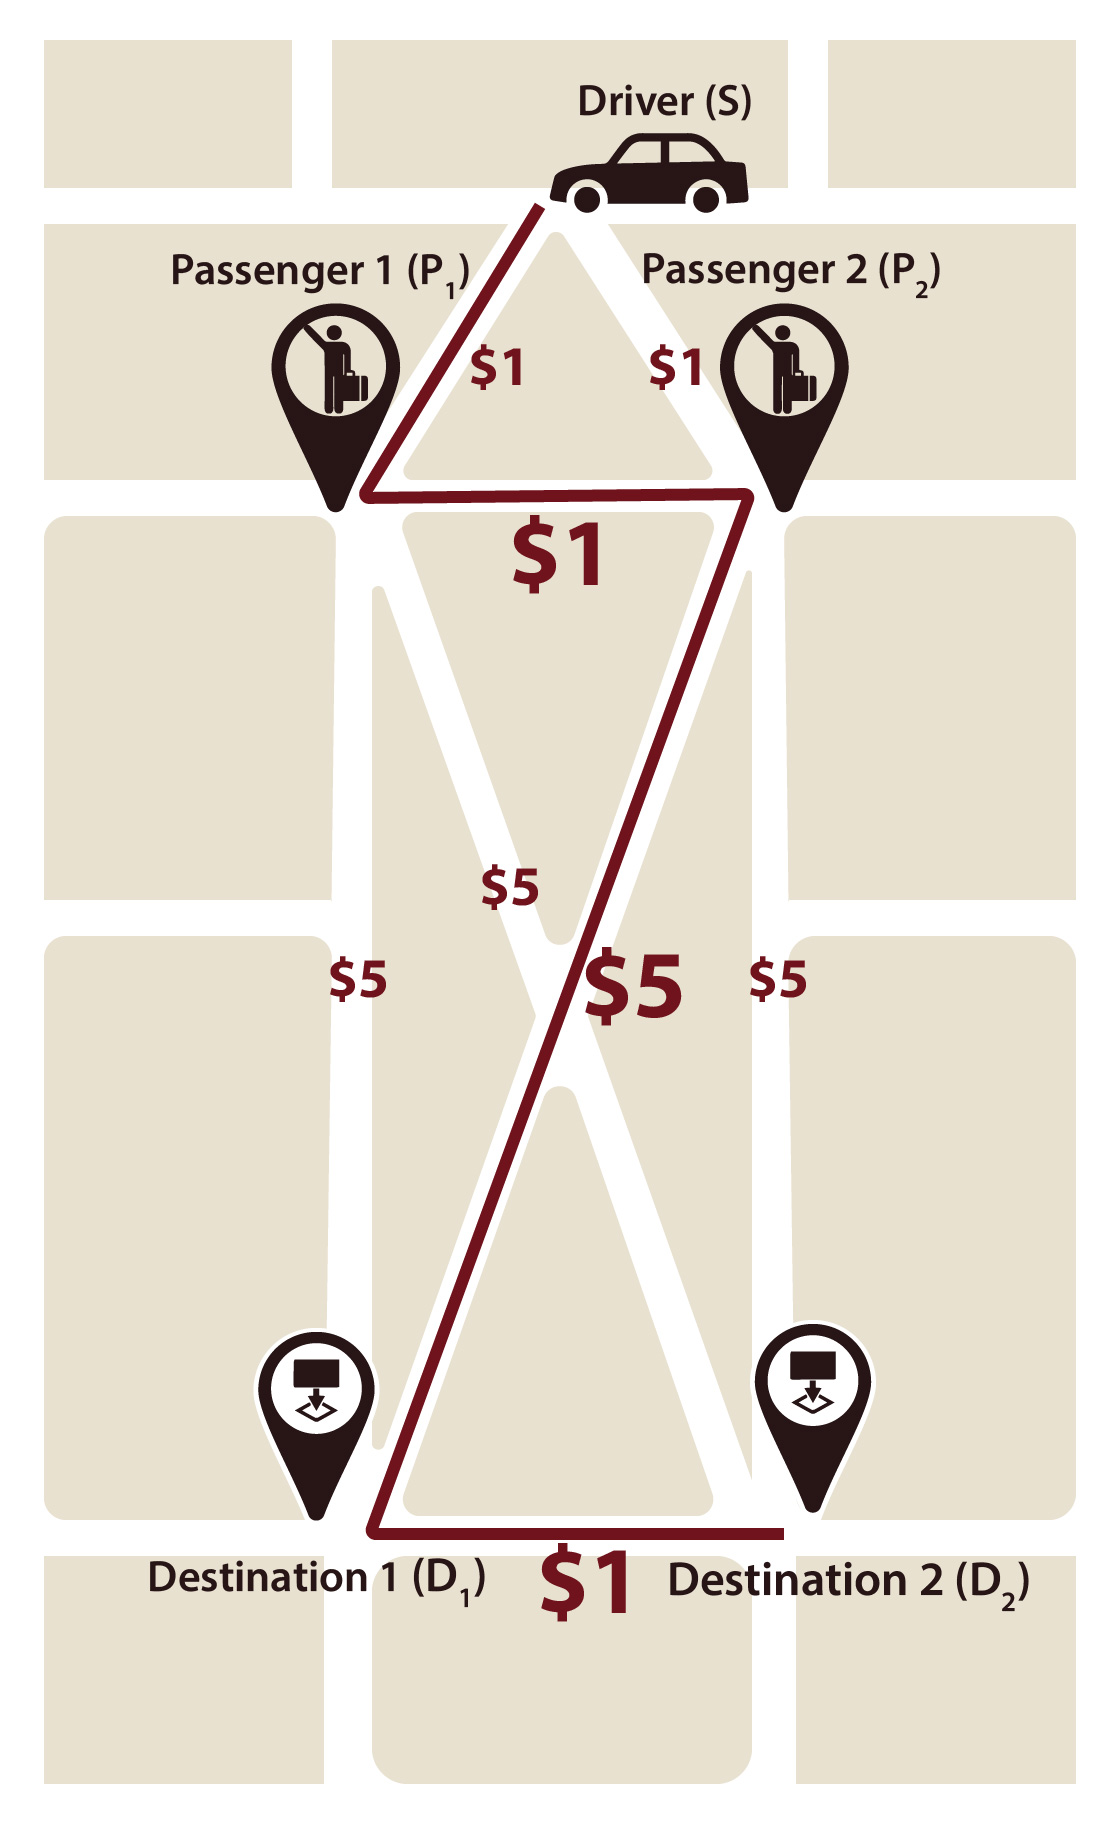
\includegraphics[width=6cm]{figures/mapV2_2.jpg}
  \caption{One of the best routing when both Passenger 1 and Passenger 2 carpool}
\end{figure}

\begin{figure}[htp]
  \centering
  \captionsetup{justification=centering}
  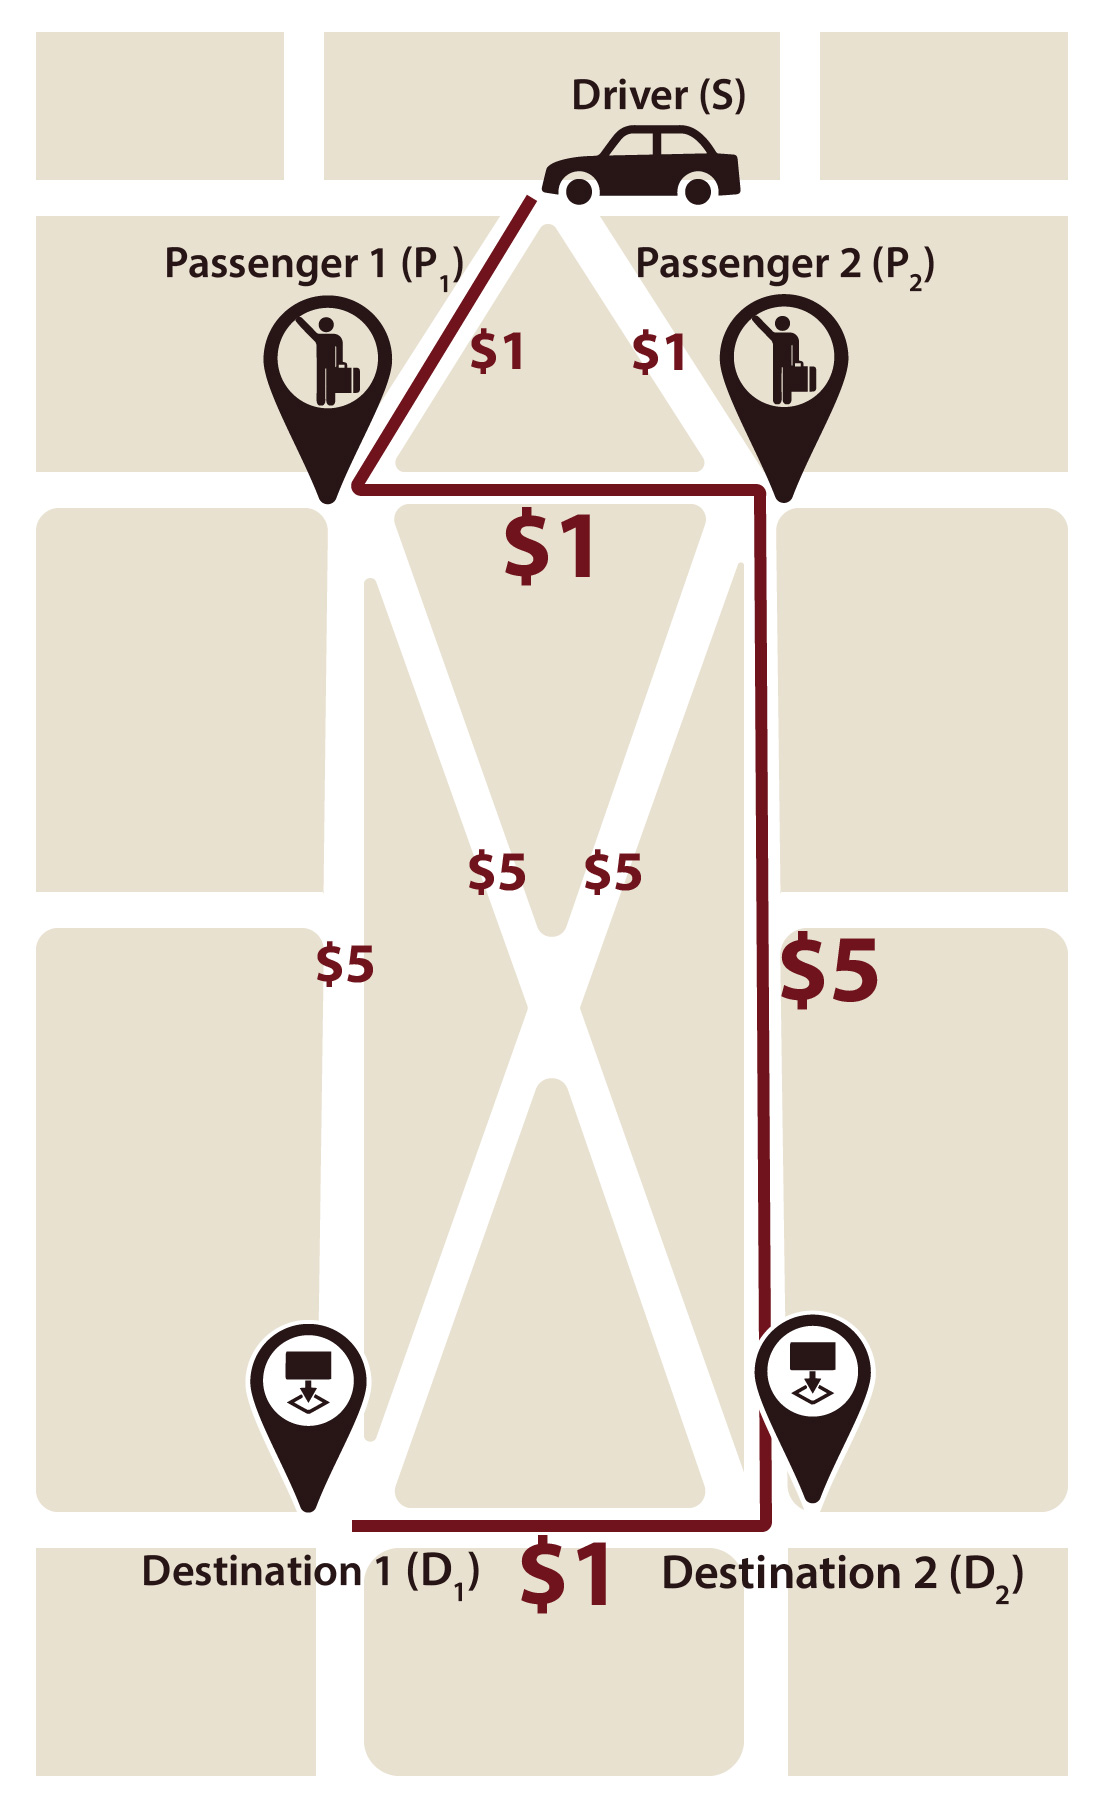
\includegraphics[width=6cm]{figures/mapV2_3.jpg}
  \caption{Another best routing when both Passenger 1 and Passenger 2 carpool}
\end{figure}
\newpage

\subsection{Fairness of Vehicle Dispatching}

In order to consider the fairness when dispatching driver, we introduce Jain's fairness index to avoid unfair situation:

$Firness\ Index = f_A(x) = \frac{\left(\sum\limits_{i=1}^{n} x_i\right)^2}{n \sum\limits_{i=1}^{n} x_i^2}$

We take accumulate driving requests that a driver has received as the metrics for fairness. That is, when a driver receives more driving requests in the past, he/she should give his/her chance of receiving a new driving request to the one who takes fewer driving requests.

As a new driving request comes, we need to ensure our system must get more or at least keep the same fairness. Hence, we form a constraint that the fairness index can not decrease compared to the previous fairness index.

However, when the driving resource changes, such as a new driver joins our system, it will violate our constraint for fairness. Because the newcomer has not taken any driving request before, the fairness will decrease. Even if a driver leaves our system, the fairness will increase or decrease due to the driver's situation. As a result, we need to reset the fairness index to the initial state and reset all the drivers' accumulated driving requests to 0. Nevertheless, it will make the fairness index's denominator to 0, which can not be divided. To avoid this situation, we assign a virtual driver with one accumulated driving request, which will make the fairness index to $\frac{1}{(n+1)}$, where $n$ is the number of drivers in our system. Moreover, for any situation that the fairness index will decrease when dispatching a new driving request, the fairness will reset.

\section{Mathematical Model}

Before we describe our mathematical model, we will go through the assumptions in the system. There are two assumption in out system:

\begin{enumerate}
  \item Every driving request only includes one passenger. This driving request will be split into multiple one-person driving request for a driving request with multiple people.
  \item System calculation time is not considered, that is, assume that drivers' location will still keep unchanged after the time of system calculation.
 \end{enumerate}

\renewcommand\arraystretch{1.5}
\par
\begin{table}[ht]
  \centering
  \caption{Notations of given parameters}
  \begin{tabularx}{\textwidth}{cX}
  \toprule
  Notation & Description \\
  \midrule
    $R$ & Set of drivers in the system (take $i$ as index) \\
    $P$ & Set of passengers in the system (take $j$ as index) \\
    $D$ & Set of destinations in the system (take $k$ as index) \\
    $L$ & Set of links on the road network \\
    $P_r$ & Set of all paths for driver $r$, where $r \in R$ \\
    $B_r$ & Set of passengers that driver $r$ has picked up, where $r \in R$ \\
    $a_l$ & The fare for the link $l$, where $l \in L$ \\
    $Q_r$ & Maximum load capacity for driver $r$, where $r \in R$ \\
    $\delta_{pl}$ & Indicator function which is 1 if link $l$ on the route $r$ is selected; 0 otherwise \\
  \bottomrule
  \end{tabularx}
\end{table}  
\par

\begin{table}[ht]
  \centering
  \caption{Notations of decision variables}
  \begin{tabularx}{\textwidth}{cX}
  \toprule
  Notation & Description \\
  \midrule
  $x_p$ & Binary variable that indicates where route $p$ is chosen, $p \in P_z$. 1 if $p$ is chosen; 0 otherwise. \\
  $y_l$ & Binary variable that indicates whether link $l$ is on the shortest path. 1 if $l$ is on the shortest path; 0 otherwise. \\
  \bottomrule
  \end{tabularx}
\end{table}  
\newpage

\subsubsection*{Objective Function}

\begin{align*}
  max\ min\ \frac{Original\ cost_i - carpool\ cost_i}{Original\ cost_i}
\end{align*}

\subsubsection*{Constraints}

\begin{align*}
  s.t. & \sum\limits_{p \in P_z} x_p = 1 && for\ v_i \ \& \ u_i, i \in \{1,2,...,n\} \tag{1} \\
  & \sum\limits_{p \in P_z} x_p \delta_{pl} = y_l && \forall l \in L \cup L' \cup L'' \tag{3} \\
  & y_l = 1 && \forall l \in L' \cup L"" \tag{4} \\
  & \sum\limits_{p \in P_w} z_p \delta_{pl} \leq y_l && \forall w \in V \cup U = W \tag{5} \\
  & \sum\limits_{p \in P_w} z_p = 1 && \forall w \in W \tag{6} \\
  & z_p = 0 \ or \ 1 \tag{7} \\
  & \sum\limits_{l \in L \cup L'} \sum\limits_{p \in Q_{v_i}} z_p \delta_{pl} a_l \leq \sum\limits_{l \in L \cup L'} \sum\limits_{p \in Q_{u_i}} z_p \delta_{pl} a_l && \forall i \in \{1,2,,...,n\} \tag{8} \\
\end{align*}

% % !TeX root = ../main.tex

\chapter{英文測試}

\section{出師表}

\lipsum

\section{短歌行}

\lipsum

This is just to test \cite{Krasnogor2004e} the cite function.

% 參考文獻
% References
\refmatter
% \normalem
\bibliographystyle{IEEEtran}
\bibliography{back/references}

% 附錄
% Appendices
% % !TeX root = ../main.tex

\appendix{A}{Introduction}
\section{Introduction}
\section{Further Introduction}

% % !TeX root = ../main.tex

\appendix{B}{Introduction}
\section{Introduction}
\section{Further Introduction}


\end{document}
